\begin{example} \label{eg:5.5.1} % EXAMPLE
Evaluate the following improper integrals.

\bmtwo
\begin{enumerate}[1)]
\item		$\ds\int_1^\infty \frac1{x^2}\ dx$
\item		$\ds\int_1^\infty \frac1{\sqrt{x}}\ dx$
\item		$\ds\int_{-\infty}^0 e^x\ dx$
\item		$\ds\int_{-\infty}^\infty \frac1{1+x^2}\ dx$
\end{enumerate}
\emtwo


\solution
\begin{enumerate}[1)]
\item	$\begin{aligned}[t] 
\int_1^\infty \frac{1}{x^2}\ dx &= \lim_{b\to\infty} \int_1^b\frac1{x^2}\ dx \\ 
&= \lim_{b\to\infty} \frac{-1}{x}\Big|_1^b \\
&= \lim_{b\to\infty} \frac{-1}{b} + 1\\
&= 1.
\end{aligned}$

A graph of the area defined by this integral is given in Figure~\ref{F:5-5-EG1}-(a).
 
\item $\begin{aligned}[t]
\int_1^\infty \frac1{\sqrt{x}}\ dx & = \lim_{b\to\infty}\int_1^b\frac1{\sqrt{x}}\ dx \\
&= \lim_{b\to\infty} 2\sqrt{x}\Big|_1^b \\
&= \lim_{b\to\infty} 2\sqrt{b}-2 \\
&= \infty.
\end{aligned}$
	
The limit does not exist, hence the improper integral $\ds\int_1^\infty\frac1x\ dx$ does not exist. %Compare the graphs in Figures \ref{fig:impint1a} and \ref{fig:impint1b}; notice how the graph of $f(x) = 1/x$ is noticeably larger. This difference is enough to cause the improper integral to diverge.

\item $\begin{aligned}[t]
\int_{-\infty}^0 e^x \ dx &= \lim_{a\to-\infty} \int_a^0e^x\ dx \\
&=  \lim_{a\to-\infty} e^x\Big|_a^0 \\
&= \lim_{a\to-\infty} e^0-e^a \\
&= 1.
\end{aligned}$
		
A graph of the area defined by this integral is given in Figure~\ref{F:5-5-EG1}-(c).

\item We will need to break this into two improper integrals and choose a value of $c \in (-\infty,\infty)$. Any value of $c$ is fine; we choose $c=0$.
\begin{align*}%
\int_{-\infty}^\infty \frac1{1+x^2}\ dx &= \lim_{a\to-\infty} \int_a^0\frac{1}{1+x^2}\ dx + \lim_{b\to\infty} \int_0^b\frac{1}{1+x^2}\ dx \\
&= \lim_{a\to-\infty} \arctan(x)\Big|_a^0 + \lim_{b\to\infty} \arctan(x)\Big|_0^b\\
\intertext{\[= \lim_{a\to-\infty} \left(\arctan(0)-\arctan(a)\right) + \lim_{b\to\infty} \left(\arctan(b)-\arctan(0)\right)\]}
&= \left(0-\frac{-\pi}2\right) + \left(\frac{\pi}2-0\right).\\
\intertext{Each	limit exists, hence the original integral converges and has value:}
&= \pi.
\end{align*}

A graph of the area defined by this integral is given in Figure~\ref{F:5-5-EG1}-(d).
\end{enumerate}
\end{example}

\begin{marginfigure}
\begin{center}
\subfloat[A graph of $f(x) = \frac{1}{x^2}$.]{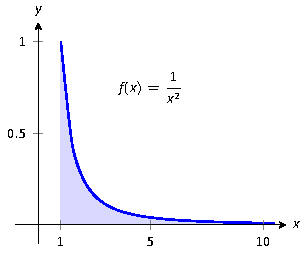
\includegraphics[scale=.75]{figures/figeximpint1a} }

\subfloat[A graph of $f(x) = \frac{1}{\sqrt{x}}$.]{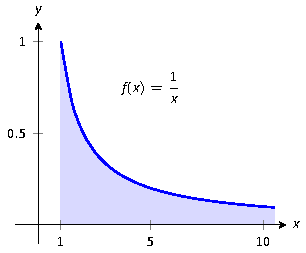
\includegraphics[scale=.75]{figures/figeximpint1b}}

\subfloat[A graph of $f(x) = e^x$.]{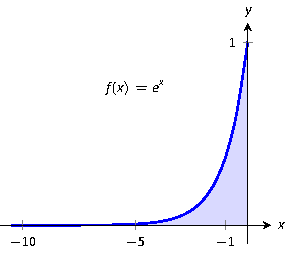
\includegraphics[scale=.75]{figures/figeximpint1c}}

\subfloat[A graph of $f(x) = \frac{1}{1+x^2}$.]{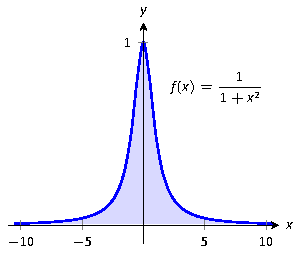
\includegraphics[scale=.75]{figures/figeximpint1d}}
\caption{The various graphs used  in Example~\ref{eg:5.5.1}.}
\label{F:5-5-EG1}
\end{center}
\end{marginfigure}